\chapter{Ways to View Stereoscopic Images}

\paragraph{} There are many ways to view Stereoscopic Images -
%\begin{enumerate}
%	\item Stereo Pairs (stereoscope: separate display for each eye)
%	\item Shutter glasses (most common method)
%	\item Color filter glasses (used in some old 3D movies)
%	\item Polarizing glasses (used in some modern 3D movies)
%\end{enumerate}
\section{Stereo Pairs}
\paragraph{} Typical stereo pair images are two separate images of the same object taken a few inches apart. In this method, the two images are not interlaced but rather presented side by side (left eye image on left and right eye image on right). The images are directly viewable using parallel "free-viewing" glasses which allow each eye to only see its corresponding image.

\section{LCD Shutter Glass Method}
\paragraph{} In the LCD shutter glass 3D display, the left and right images are alternated rapidly on the monitor screen. When the viewer looks at the screen through shuttering eyewear, each shutter is synchronized to occlude the unwanted image and transmit the wanted image. Thus each eye sees only its appropriate perspective view. The left eye sees only the left view, and the right eye only the right view.

\section{Color Filter Glasses}
\paragraph{} Color filter glasses are one of the oldest methods of viewing 3D images or movies. The system works by feeding different images into your eyes. The different color filters allow only one of the images to enter each eye, and your brain does the rest. There are two color filter systems: Red/Blue and Red/Green.

\section{Polarizing Glasses}
\paragraph{} This method is more commonly used in today's 3D movie projections. The audience must wear special glasses which have two polarizing lenses which have their polarization directions adjusted to be 90 degrees different. This makes is possible that left eye sees it's picture without problems but everything ment to right eye (sent out at different polarization) seems to be black. Same applies also to right eye.\\\\

\begin{figure}[H]
	\centering
	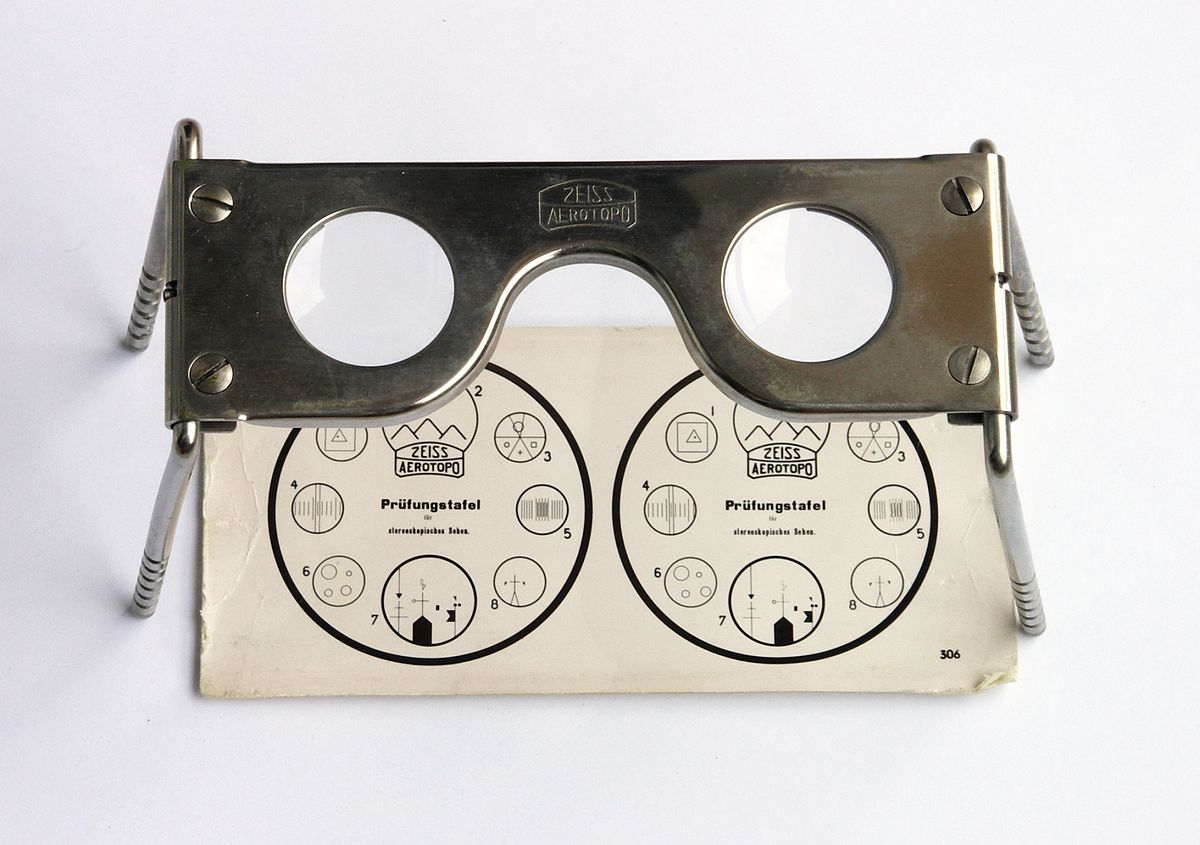
\includegraphics[height= 8cm, width=10cm]{project/images/st.jpg}
	\caption{\textsc{Stereo Glass module}}
\end{figure}

\begin{figure}[H]
	\centering
	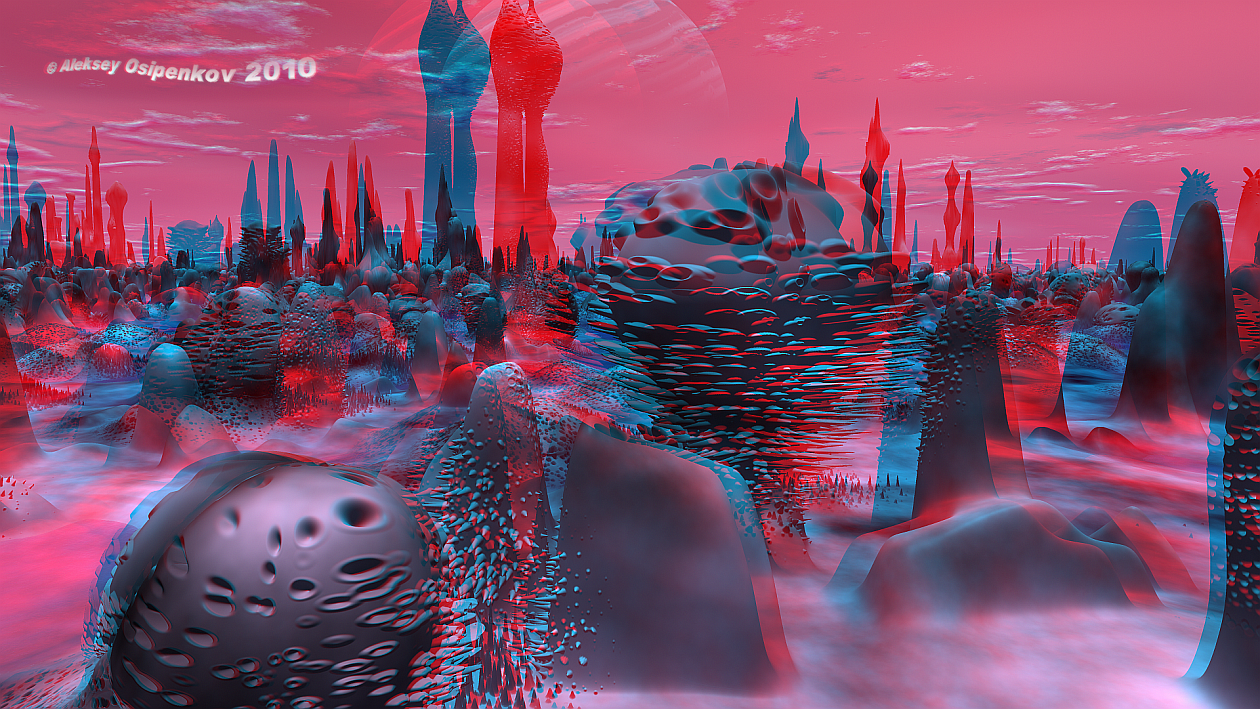
\includegraphics[height= 8cm, width=10cm]{project/images/de.png}
	\caption{\textsc{Image with 3D perception}}
\end{figure}